\documentclass[twocolumn]{NobArticle}

\usepackage{tikz}
\usetikzlibrary{positioning, shapes.geometric, arrows.meta, fit, backgrounds, calc, decorations.pathreplacing, decorations.pathmorphing}
\usepackage{subcaption}
\usepackage{listings}
\usepackage{float}
\usepackage{graphicx}
\graphicspath{{../imgs/}}

% Listings style for config snippets
\definecolor{codebg}{RGB}{248,248,248}
\definecolor{codeborder}{RGB}{210,210,210}
\definecolor{codecomment}{RGB}{80,140,80}
\definecolor{codeprompt}{RGB}{0,90,140}

\lstdefinestyle{conf}{
    basicstyle=\ttfamily\scriptsize,
    backgroundcolor=\color{codebg},
    frame=single,
    rulecolor=\color{codeborder},
    framerule=0.4pt,
    breaklines=true,
    columns=fullflexible,
    keepspaces=true,
    showstringspaces=false,
    commentstyle=\color{codecomment},
    numbers=none,
    xleftmargin=3pt,
    framexleftmargin=2pt,
    aboveskip=6pt,
    belowskip=4pt,
}
\lstset{style=conf}

% Running head and footer text
\runninghead{Practical Network Defense}
\footertext{ACME 30 A2 -- 2025/2026}

\title{ACME 30 -- Assignment no.\,2: VPN on ACME co.}

\author{
    Alberto Pulcini 2046542 \\
    Nicolò Piovan 2219663 \\
    Giovanni Colasuonno 2046000 \\
    Davide Nardoni 2060903
}

\date{\today}

\begin{document}

\maketitle
\thispagestyle{empty}

\section{Introduction}

This report describes the work carried out by our group for the second
assignment of the course. The activity was organised in the following phases:

\begin{enumerate}
    \item \textbf{Initial brainstorming}, where we discussed the goals of the
    assignment and decided where to place the VPN gateway, how to structure
    the X.509 PKI and how to enforce the per-role access policy of the four
    road-warrior accounts.
    \item \textbf{PKI and certificate setup}, in which we created the internal
    Certificate Authority and issued the server and client certificates used
    by both the OpenVPN service and the site-to-site IPSec tunnel.
    \item \textbf{Road-warriors OpenVPN}, where we configured the OpenVPN
    server on the Main firewall, defined a dedicated tunnel subnet per role
    (Alice, Bob, Christina, Diana) and wrote the firewall rules that enforce
    the access matrix required by the assignment.
    \item \textbf{Main-Internal IPSec tunnel}, in which we established an
    IPSec connection between the Main and the Internal firewalls so that the
    traffic crossing the transit link is authenticated and encrypted.
    \item \textbf{IPv6 extension}, where we replicated the same OpenVPN and
    IPSec setup over IPv6 using a ULA pool for the tunnel addresses and the
    global prefixes delegated to the ACME-30 network.
    \item \textbf{Tests}, used to validate that each road-warrior account can
    only reach the networks allowed by its role and that the site-to-site
    traffic actually flows inside the IPSec tunnel.
    \item \textbf{Final remarks}, summarising the lessons learned and the
    main difficulties encountered.
\end{enumerate}

The following sections detail each of these phases.

\section{Brainstorming}

The two main choices to make before touching any configuration were
\textit{where to terminate the road-warrior VPN} and \textit{how to map
the four user roles onto firewall rules}. The full topology is recalled
in Figure~\ref{fig:topology}.

\subsection{Where to place the OpenVPN gateway}

Per-role access (Alice $\to$ external services only, Diana $\to$ any net,
etc.) can only be enforced where the firewall sees the decrypted tunnel
traffic. We therefore terminate OpenVPN \textit{on the Main firewall}
itself, using OPNsense's built-in server: road warriors hit the public
WAN IP, the tunnel is decrypted on a \texttt{tun} interface, and from
that point on the firewall applies normal rules. A VPN box on the
internal network or in the DMZ would either hide the user identity behind
the encrypted UDP flow or force us to punch DMZ-to-internal holes, so
both options were discarded.

\subsection{Per-role addressing}

The trick used to enforce the four roles is to give each user its own
source range on the tunnel side, so that the firewall can write its
rules in terms of subnets instead of usernames. We picked the
\texttt{10.8.0.0/22} pool, split into four \texttt{/24} blocks, one per
role (Table~\ref{tab:vpnpools}). Each block is exported as a firewall
alias (\texttt{vpn\_external}, \texttt{vpn\_standard},
\texttt{vpn\_power}, \texttt{vpn\_admin}) and used in four pass rules,
closed by an explicit \textit{any\,$\to$\,any block} on the OpenVPN
interface.

\begin{table}[H]
\centering
\begin{tabular}{lll}
\toprule
\textbf{User} & \textbf{Role} & \textbf{Tunnel block} \\
\midrule
Alice     & External      & \texttt{10.8.0.0/24} \\
Bob       & Standard      & \texttt{10.8.1.0/24} \\
Christina & Power         & \texttt{10.8.2.0/24} \\
Diana     & Administrator & \texttt{10.8.3.0/24} \\
\bottomrule
\end{tabular}
\caption{One \texttt{/24} per role inside the \texttt{10.8.0.0/22} pool.}
\label{tab:vpnpools}
\end{table}

\subsection{PKI and IPSec choices}

The X.509 authentication is built around an internal CA (RSA-2048)
created on the Main firewall, which signs the OpenVPN server certificate,
one client certificate per road warrior and the two firewall certificates
used by the site-to-site tunnel. The same CA is reused for IPSec, so we
avoid PSKs and can revoke a peer by revoking its certificate. For the
IPSec Child~SAs we use narrow selectors instead of \texttt{any/any}: only
the Power and Admin VPN pools on the Main side and only the Internal
server/client networks on the other, so that a misconfigured OpenVPN
rule cannot smuggle traffic from Alice or Bob through the tunnel.

\section{PKI and certificate setup}
\label{sec:pki}

All certificates were issued from a single internal Certificate Authority
created on the Main firewall, with a 2048-bit RSA key and a 10-year
validity. The CA was then used to sign three families of certificates:

\begin{itemize}
    \item the \textit{OpenVPN server} certificate, with \texttt{Server}
    key usage, bound to the WAN address of the Main firewall;
    \item one \textit{client} certificate per road warrior (Alice, Bob,
    Christina, Diana), with the Common Name set to the username, so that
    individual revocation is possible;
    \item two \textit{IPSec server} certificates, one per firewall, with
    the IP of the transit interface declared as Subject Alternative Name
    (\texttt{100.100.254.1} for the Main and \texttt{100.100.254.2} for
    the Internal firewall), so that the peer can validate the address it
    is actually talking to.
\end{itemize}

Because the IPSec peer lives on a different appliance, the CA certificate
and the Internal firewall certificate (with its private key) were
exported as PKCS\#12 from the Main firewall and re-imported on the
Internal one. After this step both firewalls share the same trust anchor
and each one holds the private key only for its own end of the tunnel.

In addition to the X.509 mutual authentication, an OpenVPN
\textit{TLS static key} was generated and embedded in the server
configuration. It is a pre-shared HMAC that the client has to present in
the very first packet: peers that do not carry the correct key are
dropped silently, well before the TLS handshake starts, which makes
handshake-level DoS attacks much harder to mount.

\subsection{Cryptographic parameters}

All keys and channels use the OPNsense defaults, which are already a
reasonable modern baseline. The CA and every certificate it signs
(OpenVPN server, road-warrior clients, IPSec server certificates) use
\textbf{RSA-2048} as the key algorithm and \textbf{SHA-256} as the
signature digest. The OpenVPN \textit{TLS static key} is a 2048-bit
OpenVPN static-key block (PEM V1 format), used in \texttt{tls-auth}
mode as an HMAC envelope on the control channel.

For the data channel the OpenVPN server is configured with the default
OPNsense cipher list \texttt{AES-256-GCM:AES-128-GCM:CHACHA20-POLY1305}
and \textbf{SHA-256} as the auth digest~\cite{openvpn}; the negotiation
ends up on \textbf{AES-256-GCM}, an AEAD cipher that provides both
confidentiality and integrity. The TLS control channel runs on TLS\,1.2+
with the same RSA-2048 server certificate.

The IPSec connection uses IKEv2 with the OPNsense defaults too: IKE
proposal \textbf{AES-256 + SHA-256 + DH group 14} (MODP-2048), and ESP
proposal \textbf{AES-256-GCM} (128-bit ICV) with PFS on DH group 14.
IKE SA lifetime is 28800\,s, ESP SA lifetime 3600\,s, both with DPD
30/120\,s as already mentioned.

\section{Road-warriors OpenVPN}

The OpenVPN server runs on the Main firewall, bound to the WAN address
\texttt{100.100.0.2} on UDP\,1194. It uses \textit{topology subnet} over
the \texttt{10.8.0.0/22} pool described in the brainstorming and
authenticates clients with the internal CA plus the TLS static key
(cryptographic parameters listed in Section~\ref{sec:pki}).

\subsection{Per-user overrides}

Each user is bound to its own \texttt{/30} link inside the pool through a
\textit{client-specific override} that pins the tunnel network and pushes
only the routes the role is supposed to reach. The four overrides are
summarised in Table~\ref{tab:ccd}.

\begin{table}[H]
\centering
\begin{tabular}{lll}
\toprule
\textbf{User} & \textbf{Tunnel} & \textbf{Pushed routes} \\
\midrule
Alice     & \texttt{10.8.0.0/30} & ext\,(.4) \\
Bob       & \texttt{10.8.1.0/30} & DMZ\,(.6) \\
Christina & \texttt{10.8.2.0/30} & DMZ + servers\,(.1) \\
Diana     & \texttt{10.8.3.0/30} & ext, DMZ, servers, clients \\
\bottomrule
\end{tabular}
\caption{Client-specific overrides. The third column lists the third
octet of the \texttt{100.100.X.0/24} subnets pushed to the client.}
\label{tab:ccd}
\end{table}

Every override also carries the \textit{push-reset} flag, which wipes
any global \texttt{push} directive coming from the server config (including
the default \texttt{redirect-gateway}) before the per-user routes are
applied. This way each client receives \textit{only} the explicit routes
listed in its own override, and no traffic can leak through the tunnel
by inheriting a server-wide push by mistake.

\subsection{Firewall rules}

A single rule on the WAN interface lets UDP\,1194 reach the firewall
itself; everything else stays closed. On the OpenVPN interface the
access matrix is implemented as four pass rules using the four aliases
defined in Section~2.2, followed by a final default-deny rule
(Figure~\ref{fig:ovpnrules}):

\begin{itemize}
    \item \texttt{vpn\_external} $\to$ external services net (pass)
    \item \texttt{vpn\_standard} $\to$ DMZ net (pass)
    \item \texttt{vpn\_power} $\to$ DMZ + internal servers (pass)
    \item \texttt{vpn\_admin} $\to$ any (pass)
    \item any $\to$ any (block)
\end{itemize}

\begin{figure}[H]
\centering
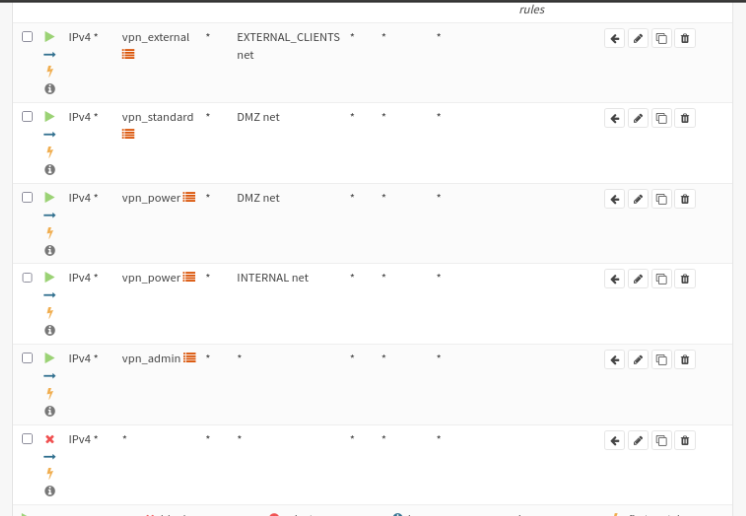
\includegraphics[width=\linewidth]{openvpn_rules.png}
\caption{OpenVPN interface rules on the Main firewall.}
\label{fig:ovpnrules}
\end{figure}

\subsection{Client connection}

Each client receives an exported \texttt{.ovpn} bundle (configuration,
CA, client certificate and TLS static key in a PKCS\#12 file) and
connects with the standard \texttt{openvpn} CLI. The handshake log for
Alice is:

\newpage
\begin{lstlisting}
$ sudo openvpn ACME_30_Roadwarriors_alice.ovpn
TCP/UDP: Preserving recently used remote
   address: [AF_INET]100.100.0.2:1194
[openvpn-server] Peer Connection Initiated
   with [AF_INET]100.100.0.2:1194
DCO device tun0 opened
net_addr_v4_add: 10.8.0.2/22 dev tun0
Initialization Sequence Completed
\end{lstlisting}

After the connection \texttt{tun0} carries the expected \texttt{/30}
endpoint inside Alice's block and the kernel only installs the routes
for the external services network, exactly as planned in the override.

\subsection{Access matrix verification}

To check that the firewall actually enforces the access matrix we ran a
pair of pings from Alice's laptop through \texttt{tun0}: one toward
\texttt{100.100.4.1} (external services, allowed) and one toward
\texttt{100.100.2.1} (clients network, denied):

\begin{lstlisting}
$ ping -I tun0 100.100.4.1
64 bytes from 100.100.4.1:
   icmp_seq=1 ttl=64 time=25.7 ms
64 bytes from 100.100.4.1:
   icmp_seq=2 ttl=64 time=25.7 ms
3 packets transmitted, 3 received,
   0% packet loss

$ ping -I tun0 100.100.2.1
4 packets transmitted, 0 received,
   100% packet loss
\end{lstlisting}

The first ping succeeds, the second one is silently dropped by the
\textit{any\,$\to$\,any block} on the OpenVPN interface, confirming that
Alice's role is correctly enforced. The same test was repeated for each
of the other three accounts and in every case only the subnets allowed
by the role answered the probes.

\subsection{Encryption check with Wireshark}

To make sure that the tunnel is actually doing its job we captured the
same Alice ping toward \texttt{100.100.4.1} on two different interfaces:
\texttt{tap0}, which is the simulated physical link to the Internet (where
the OpenVPN-encapsulated UDP packets flow), and \texttt{tun0}, which is the
in-kernel side of the decrypted tunnel.

On \texttt{tap0}, filtering with \texttt{udp.port == 1194}, Wireshark
sees only OpenVPN UDP datagrams whose payload is opaque
(Figure~\ref{fig:tap0ovpn}); no ICMP frame is ever recognised on this
interface.

\begin{figure}[H]
\centering
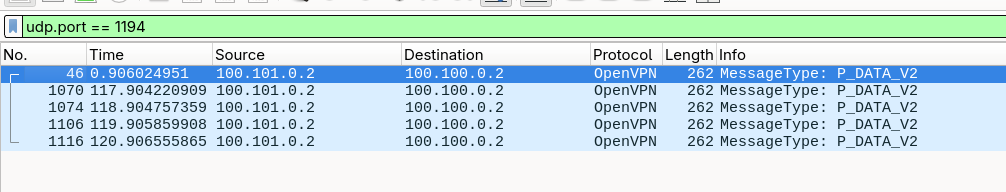
\includegraphics[width=\linewidth]{tap0_scan_ping.png}
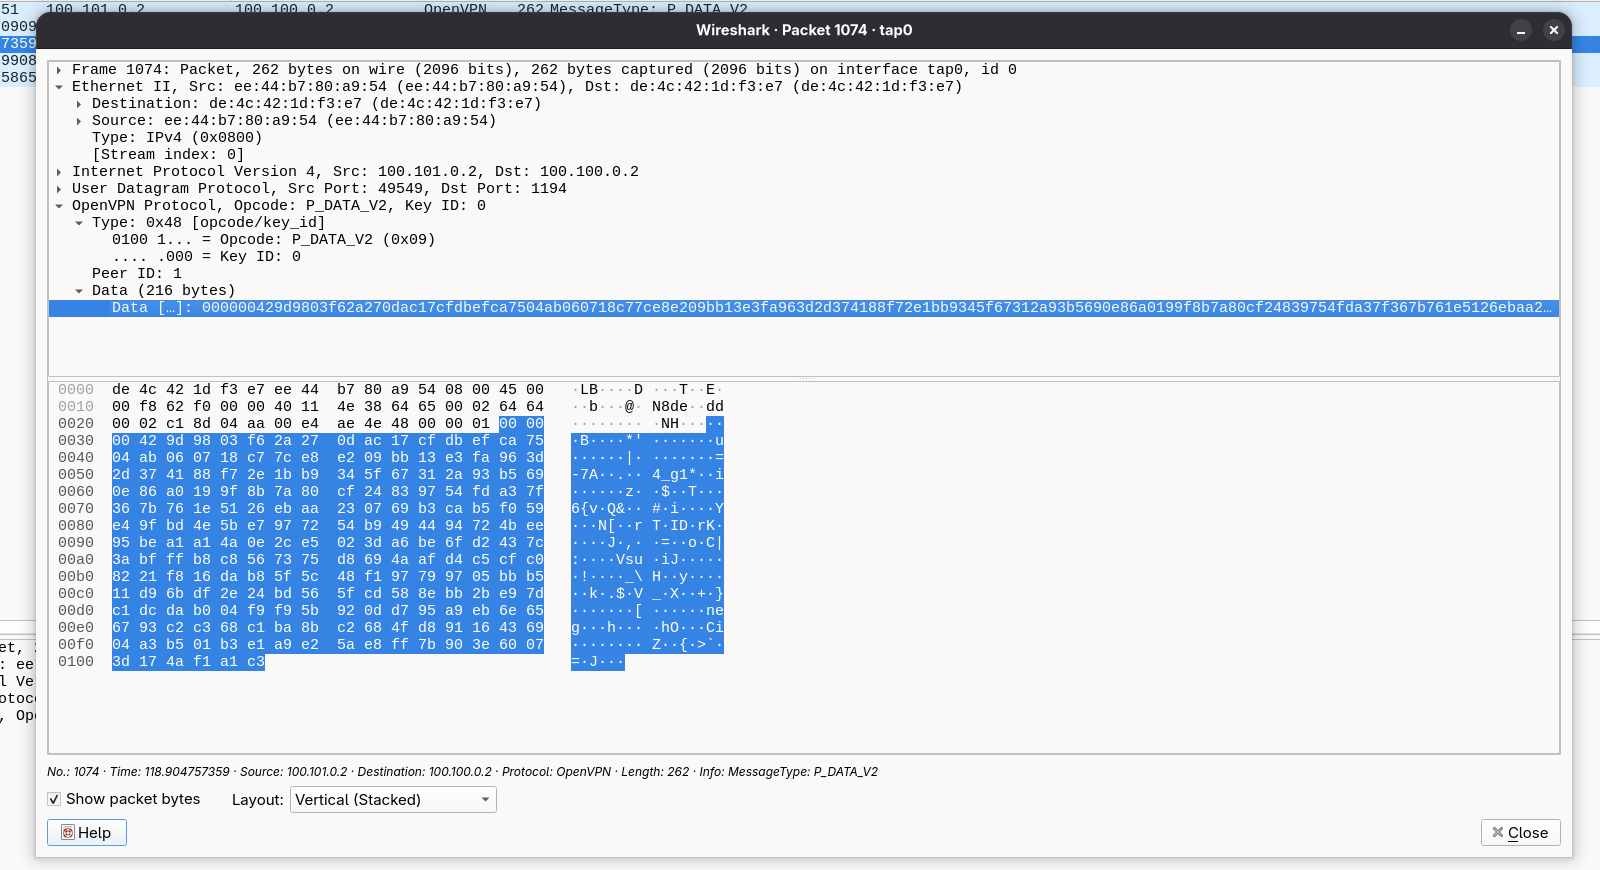
\includegraphics[width=\linewidth]{tap0_scan_bytes.png}
\caption{Capture on \texttt{tap0} during Alice's ping: only OpenVPN
UDP\,1194 datagrams with random-looking payload.}
\label{fig:tap0ovpn}
\end{figure}

On \texttt{tun0}, instead, Wireshark sees the cleartext ICMP echo
request/reply pair toward \texttt{100.100.4.1} with the expected
payload (Figure~\ref{fig:tun0ovpn}), confirming that the firewall
decrypts the traffic only on the tunnel side and that the simulated
Internet only ever observes the encrypted OpenVPN flow.

\begin{figure}[H]
\centering
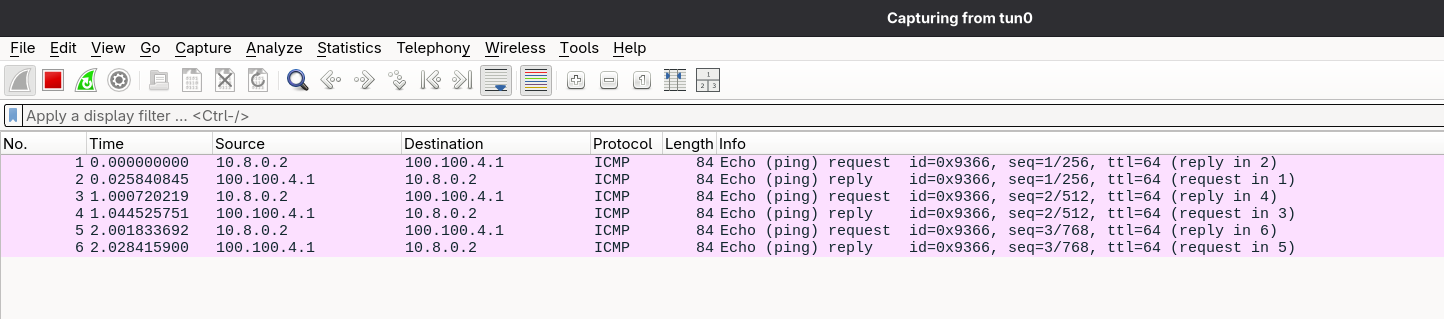
\includegraphics[width=\linewidth]{tun0_scan_ping.png}
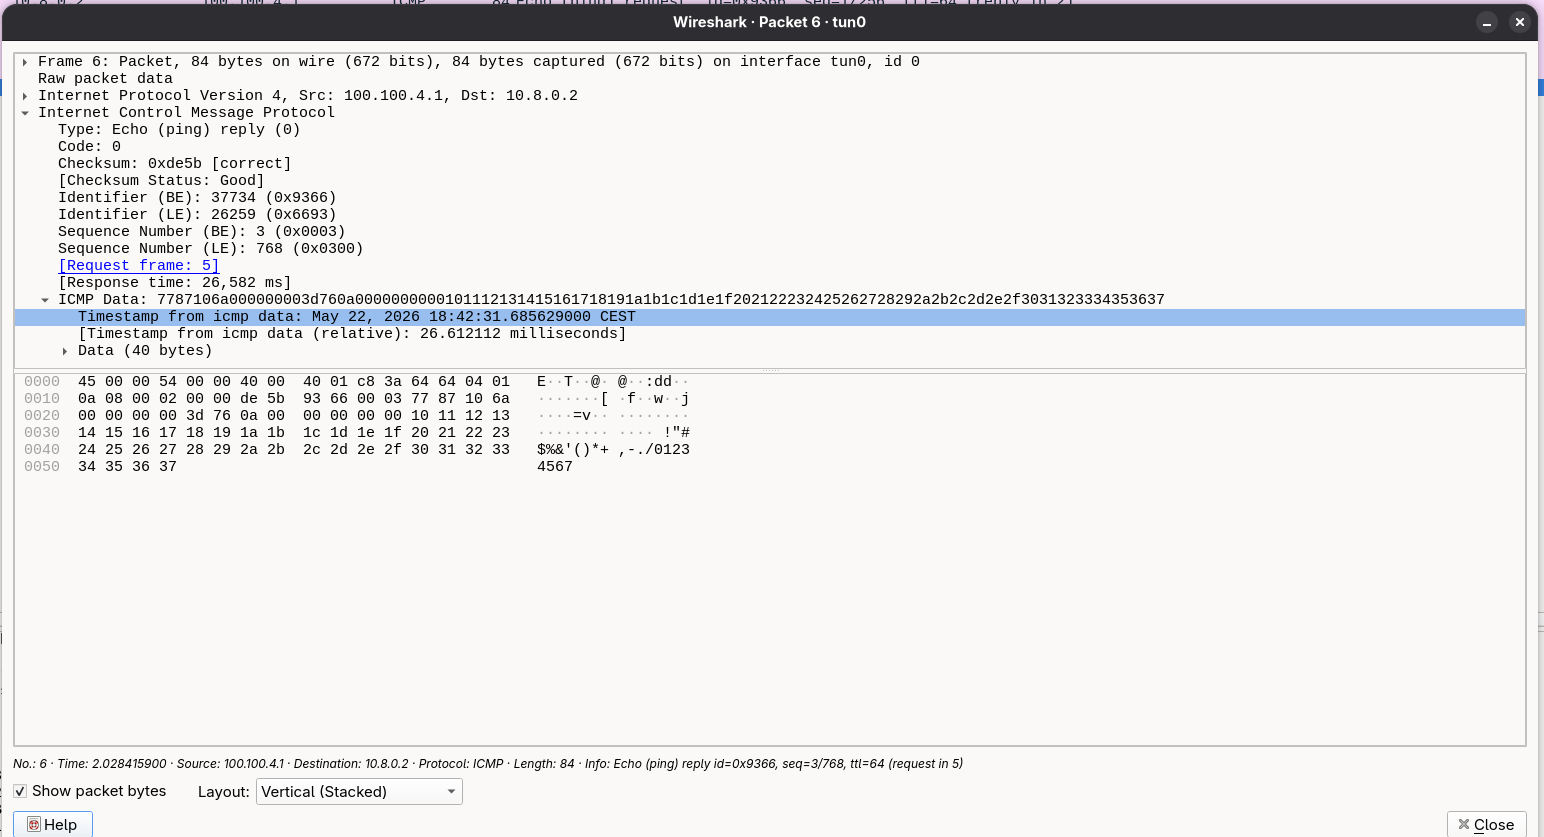
\includegraphics[width=\linewidth]{tun0_scan_bytes.png}
\caption{Same ping captured on \texttt{tun0}: cleartext ICMP echo
request/reply with readable payload.}
\label{fig:tun0ovpn}
\end{figure}

\section{Main--Internal IPSec tunnel}

The site-to-site tunnel is an IKEv2 IPSec connection between the
\texttt{100.100.254.1} interface of the Main firewall and the
\texttt{100.100.254.2} interface of the Internal one. Both peers
authenticate each other with the certificates issued in
Section~\ref{sec:pki}\footnote{Reusing the same CA created for OpenVPN.}
and run Dead Peer Detection with a 30\,s delay and a 120\,s timeout, so
that a half-broken tunnel is renegotiated automatically. Cipher suites
are the OPNsense defaults summarised in Section~\ref{sec:pki}.

\subsection{Child SAs}

The Child SAs use narrow traffic selectors instead of \texttt{any/any},
so that the tunnel only carries the traffic that the role-based policy
allows to reach the Internal site:

\begin{itemize}
    \item Main side: local \texttt{10.8.2.0/24}, \texttt{10.8.3.0/24}
    (Power + Admin VPN pools);\\
    remote \texttt{100.100.1.0/24}, \texttt{100.100.2.0/24} (Internal
    servers + Clients).
    \item Internal side: the same pairs, mirrored.
\end{itemize}

Even if a future bug in the OpenVPN ruleset let Alice or Bob send a
packet toward an internal address, IPSec would refuse to encapsulate it,
since the source would not match any selector.

\subsection{Firewall rules}

The Power pool is only allowed to reach the internal servers alias
(\texttt{internal\_server\_net} $\equiv$ \texttt{100.100.1.0/24}), while
the Admin pool can reach anything. On the Internal firewall the same
two aliases (\texttt{vpn\_power}, \texttt{vpn\_admin}) are recreated and
used to write the symmetric pass rules that let the internal hosts
answer back. Table~\ref{tab:ipsecrules} reports the complete ruleset on
the IPSec interface of both firewalls.

\begin{table}[H]
\centering
\begin{tabular}{lll}
\toprule
\textbf{FW} & \textbf{Source} & \textbf{Destination} \\
\midrule
Main     & \texttt{vpn\_power} & \texttt{internal\_server\_net} \\
Main     & \texttt{vpn\_admin} & any \\
\midrule
Internal & \texttt{internal\_server\_net} & \texttt{vpn\_power} \\
Internal & \texttt{vpn\_power}            & \texttt{internal\_server\_net} \\
Internal & any                            & \texttt{vpn\_admin} \\
Internal & \texttt{vpn\_admin}            & any \\
\bottomrule
\end{tabular}
\caption{IPSec pass rules on both firewalls. Everything else is dropped
by the implicit default-deny.}
\label{tab:ipsecrules}
\end{table}

\subsection{Connection status}

After applying the configuration on both peers the IKE Security
Association and both Child SAs come up cleanly
(Figure~\ref{fig:ipsecconn}), and the OpenVPN dashboard shows the
expected road-warrior sessions (Figure~\ref{fig:ovpnconn}).

\begin{figure}[H]
\centering
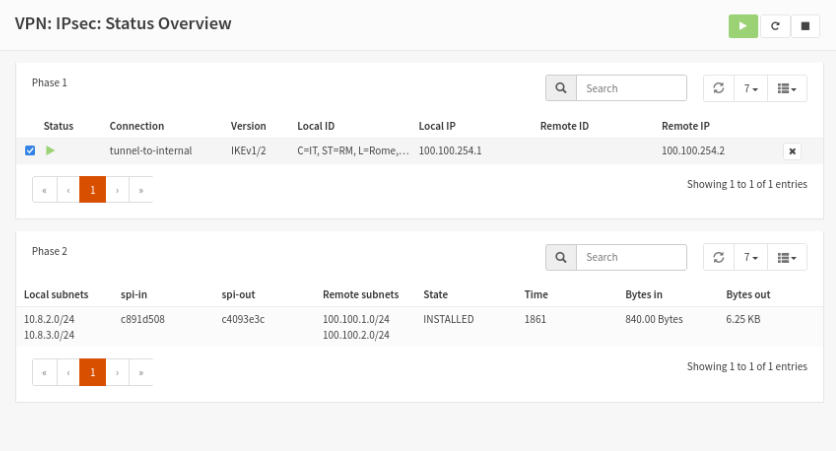
\includegraphics[width=\linewidth]{ipsec_conn.png}
\caption{IPSec status overview on the Main firewall.}
\label{fig:ipsecconn}
\end{figure}

\begin{figure}[H]
\centering
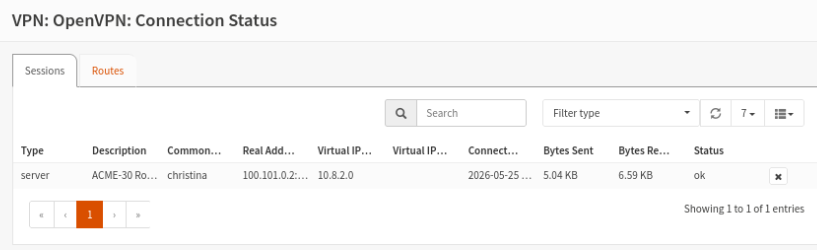
\includegraphics[width=\linewidth]{ovpn_conn.png}
\caption{OpenVPN active sessions.}
\label{fig:ovpnconn}
\end{figure}

\subsection{End-to-end test}

To exercise both VPNs at once we logged in as Christina (Power) and
pinged the DNS server inside the Internal servers network:

\begin{lstlisting}
$ ping -I tun0 100.100.1.2
64 bytes from 100.100.1.2:
   icmp_seq=1 ttl=62 time=31.0 ms
64 bytes from 100.100.1.2:
   icmp_seq=2 ttl=62 time=30.0 ms
3 packets transmitted, 3 received,
   0% packet loss
\end{lstlisting}

The packet path can be observed at three different points. On the
laptop's \texttt{tap0} interface only OpenVPN UDP\,1194 traffic is
visible (Figure~\ref{fig:ipsectap0}): nothing reveals the real IPs of
the internal server or of the firewall transit link.

\begin{figure}[H]
\centering
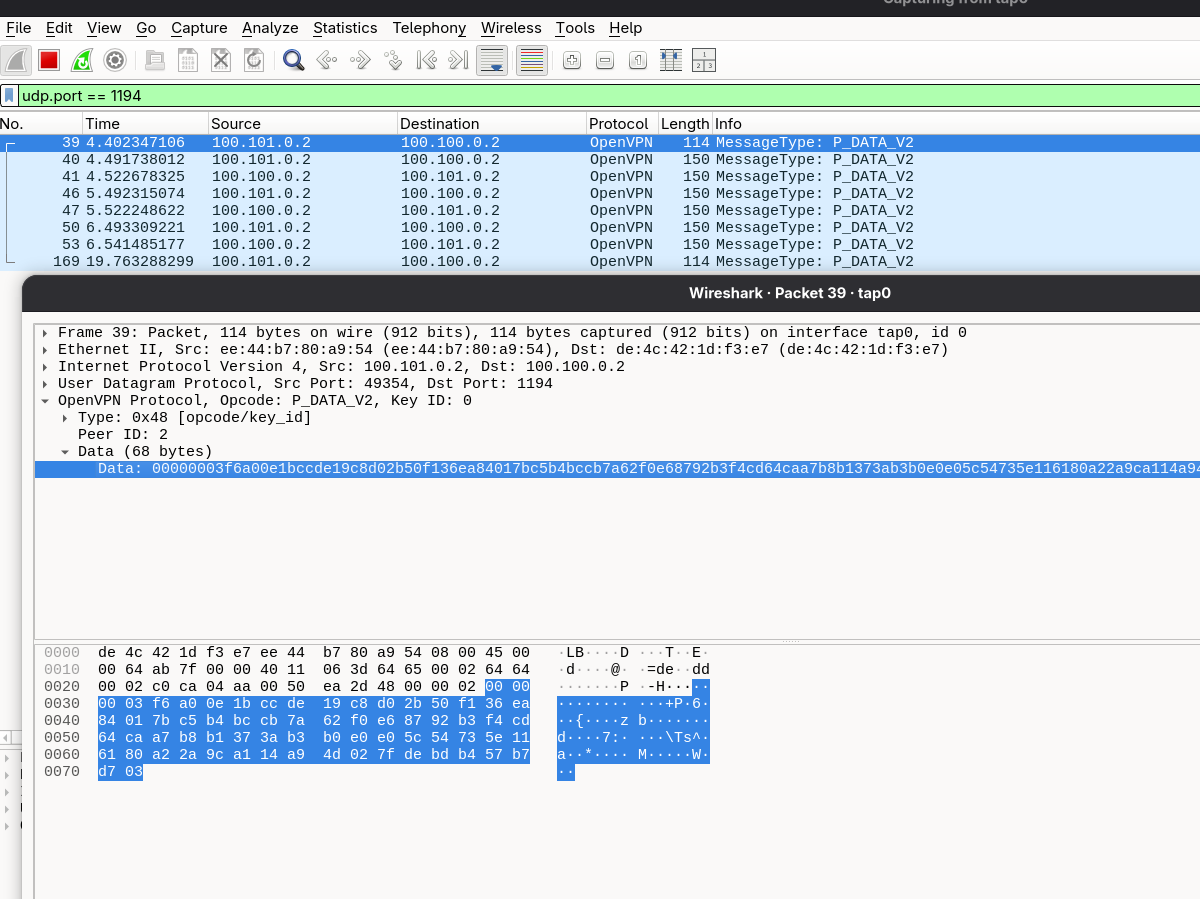
\includegraphics[width=\linewidth]{ipsec_tap0_ping.png}
\caption{\texttt{tap0} capture during Christina's ping: only the outer
OpenVPN flow is visible.}
\label{fig:ipsectap0}
\end{figure}

After OpenVPN decryption on the Main firewall the packet enters the
IPSec tunnel toward the Internal firewall. Capturing on the transit
interface of the Main firewall we see only ESP (protocol 50) packets,
with no readable inner header (Figure~\ref{fig:ipsecesp}). Finally, on
Christina's \texttt{tun0} interface the original ICMP exchange is fully
readable (Figure~\ref{fig:ipsectun0}).

\begin{figure}[H]
\centering
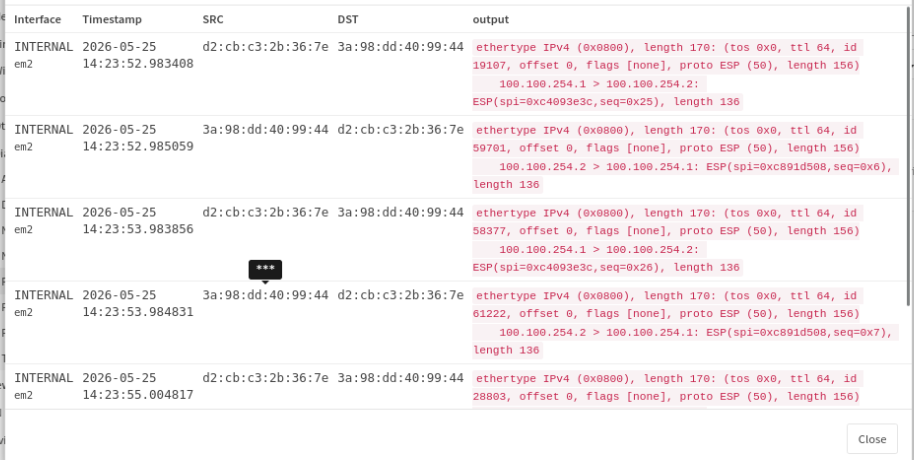
\includegraphics[width=\linewidth]{ipsec_mainfirewall_internal_int.png}
\caption{Capture on the Main firewall's transit interface: only ESP
packets toward \texttt{100.100.254.2}.}
\label{fig:ipsecesp}
\end{figure}

\begin{figure}[H]
\centering
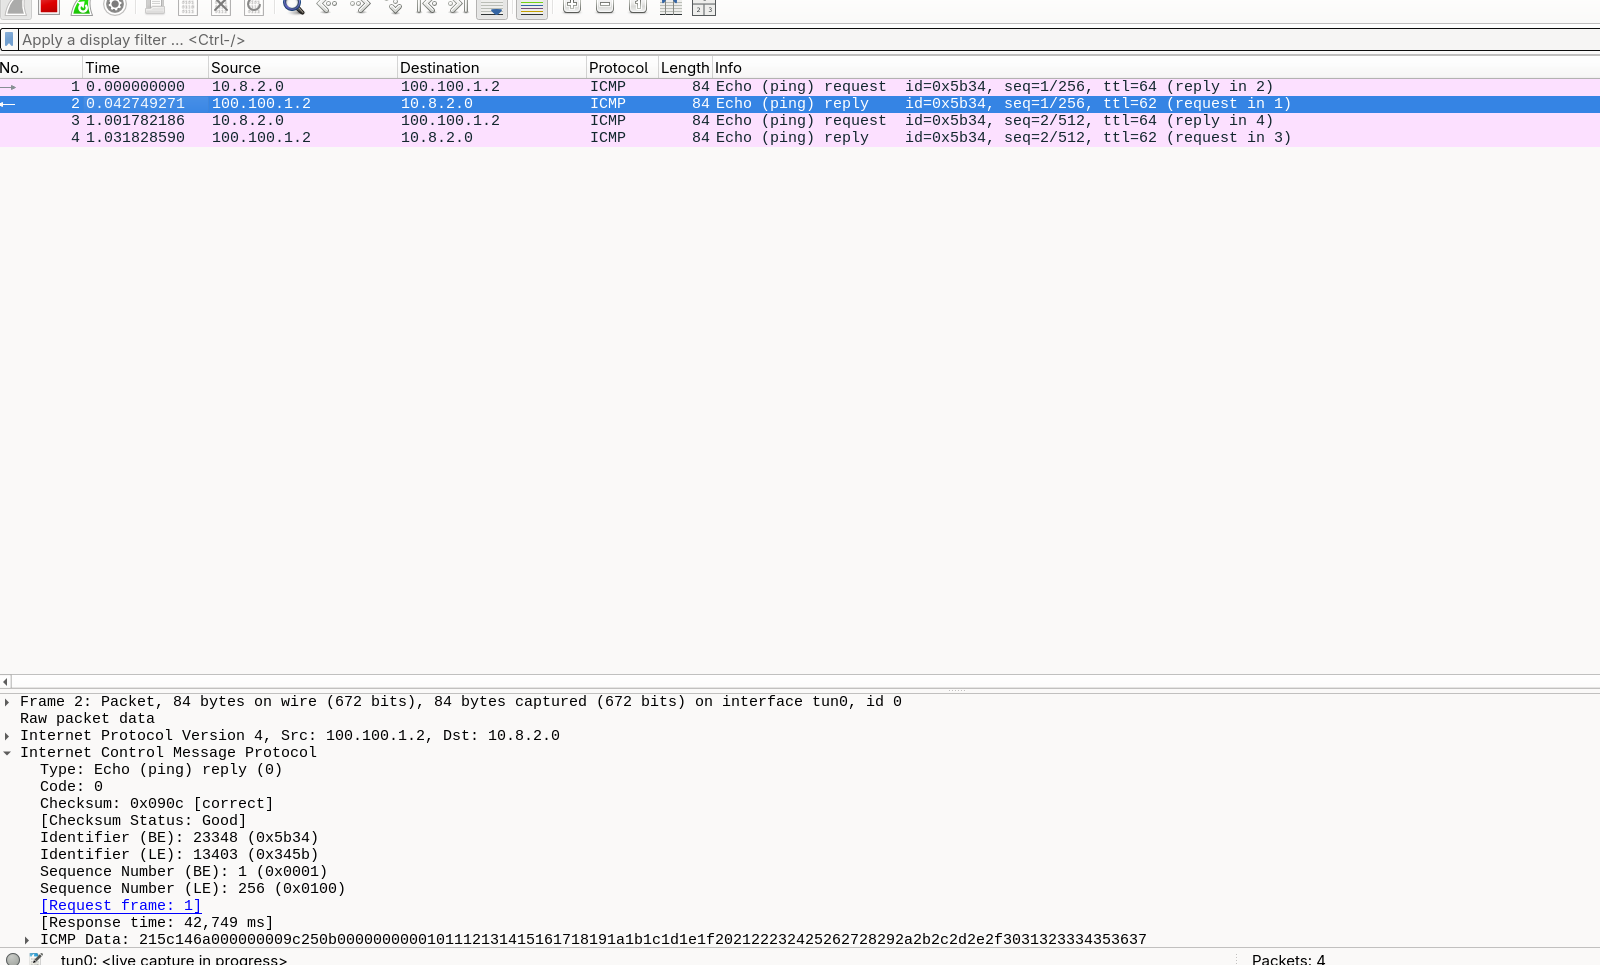
\includegraphics[width=\linewidth]{ipsec_tun0_ping.png}
\caption{Same ping seen on Christina's \texttt{tun0}: cleartext ICMP.}
\label{fig:ipsectun0}
\end{figure}

A traceroute from Christina toward the same DNS server makes the
behaviour of the two stacked tunnels explicit:

\begin{lstlisting}
$ traceroute 100.100.1.2
 1  10.8.0.1            32.4 ms
 2  * * *
 3  100.100.1.2         60.0 ms
\end{lstlisting}

Hop\,1 is the OpenVPN gateway on the Main firewall; hop\,2 is invisible
because the packet is encapsulated in ESP and the intermediate router
does not decrement the TTL on the tunnel interface; hop\,3 is the final
destination. The silent intermediate hop is the behavioural signature
of the IPSec tunnel.

\section{IPv6 extension}

Since the ACME-30 network is dual-stack from Assignment~1, we replicated
the whole VPN stack on IPv6 as well. The design mirrors the IPv4 one:
ULA pool \texttt{fd00:8::/64} split into four \texttt{/112} blocks (one
per role) for the OpenVPN tunnel, and the same IPSec connection extended
with a second pair of selectors over the global IPv6 transit addresses.

\subsection{OpenVPN IPv6}

The OpenVPN server gets \texttt{fd00:8::/64} as its IPv6 network, and
each user receives a \texttt{/112} link inside the pool through the same
client-specific override mechanism used on IPv4
(Table~\ref{tab:ccdv6}). The pushed local networks are the global
\texttt{2001:470:b5b8:1e\textit{XX}::/64} prefixes assigned to the
corresponding IPv4 subnets in Assignment~1.

\begin{table}[H]
\centering
\begin{tabular}{lll}
\toprule
\textbf{User} & \textbf{Tunnel} & \textbf{Pushed prefix} \\
\midrule
Alice     & \texttt{fd00:8::0:0/112} & \texttt{1e04::/64} \\
Bob       & \texttt{fd00:8::1:0/112} & \texttt{1e06::/64} \\
Christina & \texttt{fd00:8::2:0/112} & \texttt{1e06::/64} + \texttt{1e81::/64} \\
Diana     & \texttt{fd00:8::3:0/112} & all \\
\bottomrule
\end{tabular}
\caption{Client-specific overrides on IPv6. Prefixes are abbreviated
removing the common \texttt{2001:470:b5b8:} part.}
\label{tab:ccdv6}
\end{table}

The four \texttt{/112} blocks are exported as IPv6 firewall aliases
(\texttt{vpn\_external\_v6}, \texttt{vpn\_standard\_v6},
\texttt{vpn\_power\_v6}, \texttt{vpn\_admin\_v6}), plus a dedicated
\texttt{internal\_server\_net\_v6} for the \texttt{1e81::/64} prefix,
and used in the same role-based pass rules as IPv4 followed by a final
default-deny.

\subsection{IPv4-encapsulated IPv6}

The OpenVPN instance was configured with \texttt{proto udp4} on
UDP\,1194, so the IPv6 tunnel traffic is carried inside IPv4 OpenVPN
datagrams: on \texttt{tap0} Wireshark sees IPv4 packets with an
encrypted OpenVPN payload (Figure~\ref{fig:v6tap0}), while on
\texttt{tun0} the same packet appears as a raw IPv6 datagram with a
cleartext ICMPv6 echo inside (Figure~\ref{fig:v6tun0}). This is not a
problem for the security goal --- the payload is still protected by
OpenVPN --- it only means that the outer transport is IPv4.

\begin{figure}[H]
\centering
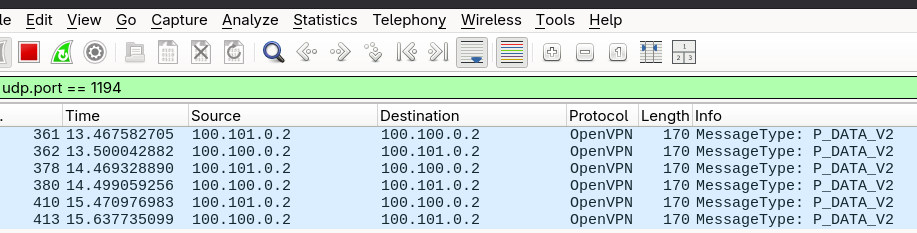
\includegraphics[width=\linewidth]{v6enc_tap0.png}
\caption{\texttt{tap0}: the IPv6 ping is carried inside IPv4 OpenVPN
datagrams on UDP\,1194.}
\label{fig:v6tap0}
\end{figure}

\begin{figure}[H]
\centering
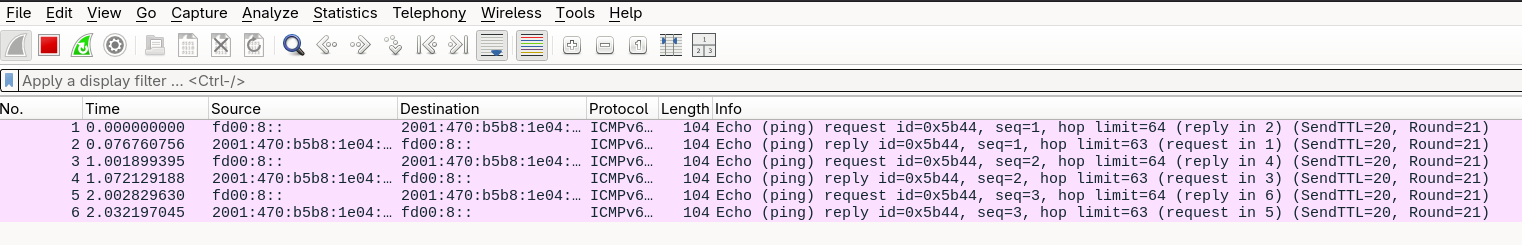
\includegraphics[width=\linewidth]{v6_enc_tun0.png}
\caption{\texttt{tun0}: same packet decapsulated, plain IPv6 ICMPv6
echo request.}
\label{fig:v6tun0}
\end{figure}

\subsection{Per-role test on IPv6}

Connected with Alice's certificate, \texttt{tun0} receives the expected
\texttt{fd00:8::/112} endpoint and an IPv6 route only toward the
external services prefix:

\begin{lstlisting}
inet6 fd00:8::/112 scope global
inet6 2001:470:b5b8:1e04::/64 dev tun0
   metric 200 pref medium
\end{lstlisting}

A ping toward an external client succeeds, while the same probe toward
the DMZ webserver returns \texttt{Network is unreachable}, because the
override did not push that route. Forcing the route manually with
\texttt{ip -6 route add 2001:470:b5b8:1e06::/64 dev tun0} the host
generates the packet, but the firewall correctly drops it (100\,\%
loss), confirming that the IPv6 rules enforce the access matrix
independently of the client-side routing table.

\subsection{IPSec IPv6}

The site-to-site tunnel was extended by adding a second child to the
existing IPSec connection, this time between the global IPv6 transit
addresses (\texttt{2001:470:b5b8:1e0f:d0cb:c3ff:fe2b:367e} on the Main,
\texttt{2001:470:b5b8:1e0f::2} on the Internal). The new selectors carry
only the Power and Admin v6 pools toward the Internal v6 prefixes:

\begin{itemize}
    \item Local: \texttt{fd00:8::2:0/112},
    \texttt{fd00:8::3:0/112}.
    \item Remote: \texttt{2001:470:b5b8:1e81::/64},
    \texttt{2001:470:b5b8:1e82::/64}.
\end{itemize}

The settings are mirrored on the Internal firewall and the dual-stack
connection comes up cleanly (Figure~\ref{fig:ipsecinternal}). The
corresponding IPSec firewall rules on both peers are shown in
Figures~\ref{fig:ipsecrules}--\ref{fig:ipsecrulescli}.

\begin{figure}[H]
\centering
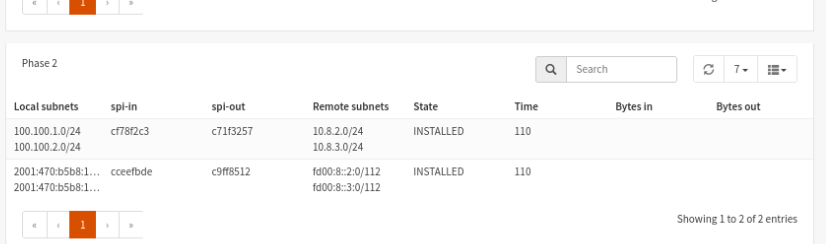
\includegraphics[width=\linewidth]{ipsec_internal.png}
\caption{IPSec status on the Internal firewall after adding the IPv6
child.}
\label{fig:ipsecinternal}
\end{figure}

\begin{figure}[H]
\centering
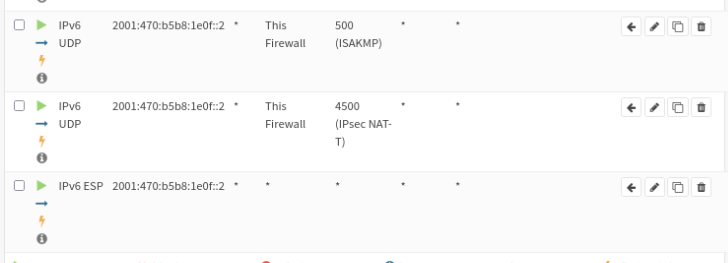
\includegraphics[width=\linewidth]{ipsec_rules.png}
\caption{IPSec firewall rules on the Main firewall.}
\label{fig:ipsecrules}
\end{figure}

\begin{figure}[H]
\centering
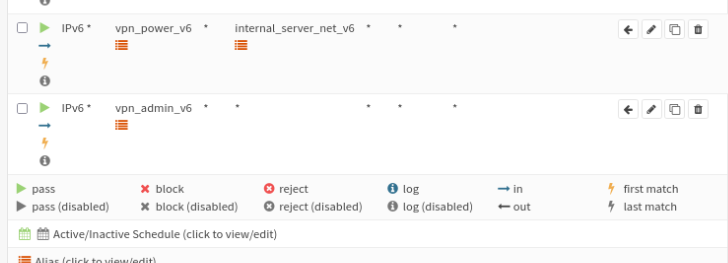
\includegraphics[width=\linewidth]{ipsec_rules_clients.png}
\caption{IPSec firewall rules on the Internal firewall.}
\label{fig:ipsecrulescli}
\end{figure}

\subsection{End-to-end IPv6 test}

Connected with Christina's certificate, a ping toward the DNS server's
global IPv6 succeeds end-to-end:

\begin{lstlisting}
$ ping -6 -I tun0
   2001:470:b5b8:1e81:4730:4341:85e8:4a85
64 bytes ... icmp_seq=1 time=123 ms
64 bytes ... icmp_seq=2 time=100 ms
64 bytes ... icmp_seq=3 time=108 ms
3 packets transmitted, 3 received,
   0% packet loss
\end{lstlisting}

The same test was repeated with Diana's certificate, capturing the
packet at three different points. On the laptop's \texttt{tap0} only the
encrypted OpenVPN flow is visible (Figure~\ref{fig:v6ipsectap0}); on
the Main firewall's transit interface only ESP packets are seen
(Figure~\ref{fig:v6ipsecesp}); on Diana's \texttt{tun0} the original
ICMPv6 echo is fully readable.

\begin{figure}[H]
\centering
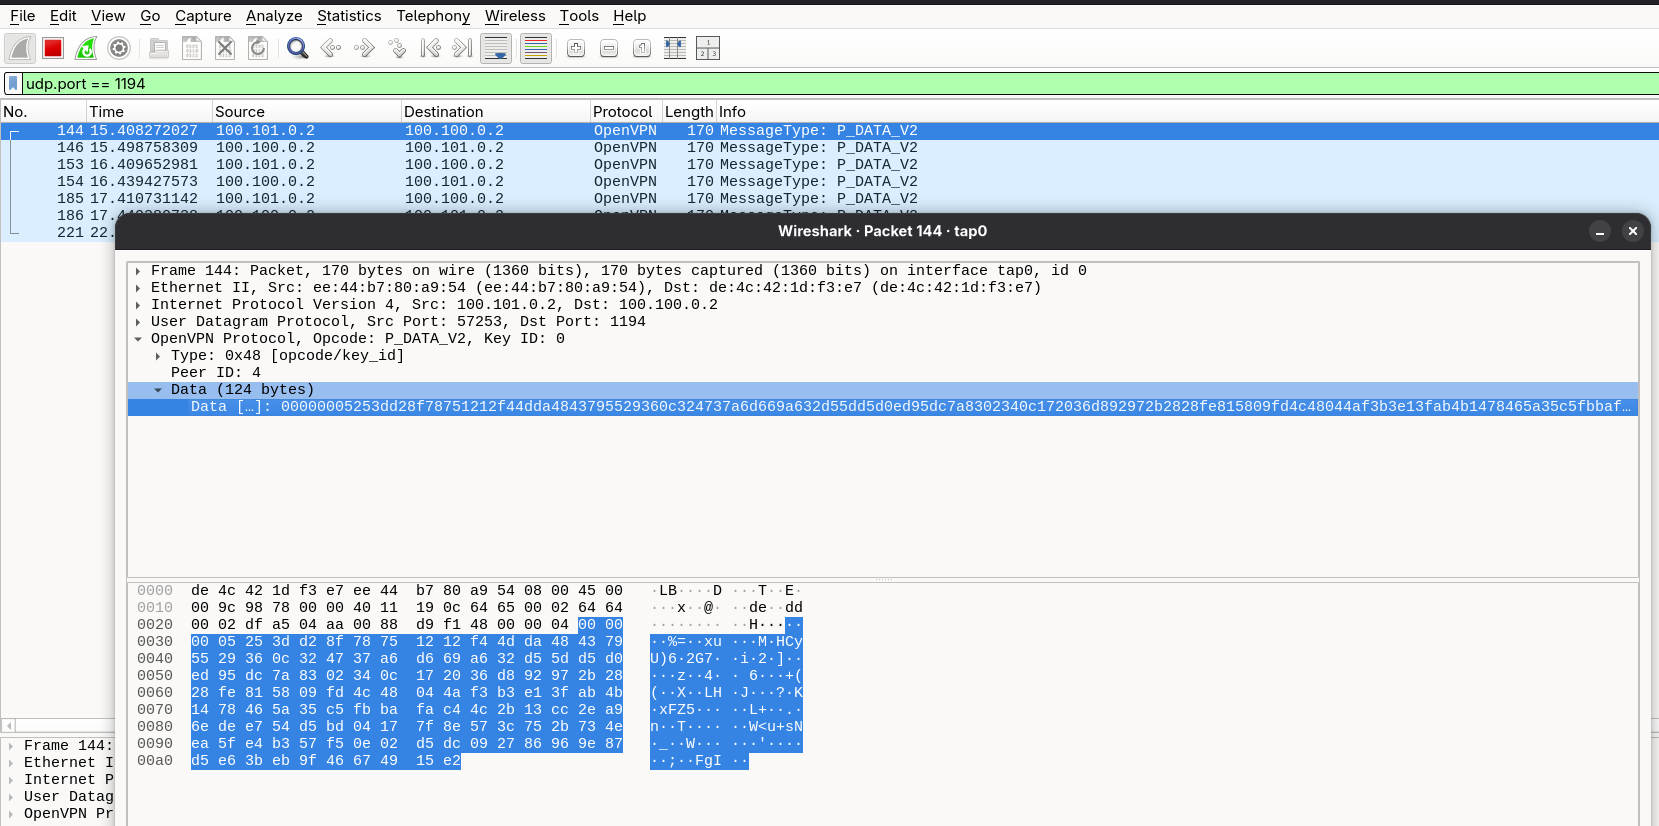
\includegraphics[width=\linewidth]{ipsec_enc_tap0.png}
\caption{Diana's ping seen on \texttt{tap0}: encrypted OpenVPN UDP
flow.}
\label{fig:v6ipsectap0}
\end{figure}

\begin{figure}[H]
\centering
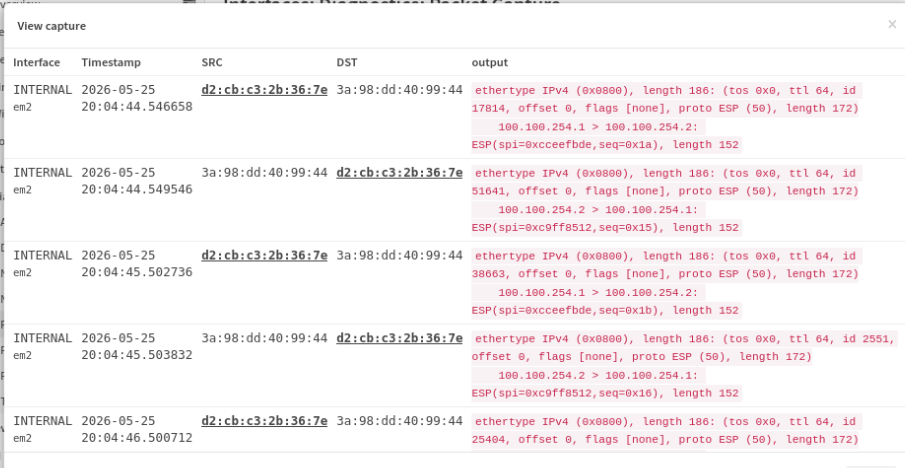
\includegraphics[width=\linewidth]{ipsec_enc_mainfirewalltointernal.png}
\caption{Same ping captured on the Main firewall's transit interface:
only ESP packets.}
\label{fig:v6ipsecesp}
\end{figure}

The traceroute confirms the two stacked tunnels exactly as on IPv4:

\begin{lstlisting}
$ traceroute -6
   2001:470:b5b8:1e81:4730:4341:85e8:4a85
 1  fd00:8::1     43.5 ms
 2  * * *
 3  2001:470:b5b8:1e81:...   43.4 ms
\end{lstlisting}

Hop\,1 is the OpenVPN gateway on the Main firewall, hop\,2 is the
IPSec-encrypted transit (invisible to traceroute), hop\,3 is the DNS
server itself.

\section{Final remarks}

The two VPN services were brought up successfully on both address
families. The road-warriors OpenVPN~\cite{openvpn} terminates on the
Main firewall and authenticates the four accounts through an internal
X.509 PKI~\cite{rfc5280}; the per-user \texttt{/30}+\texttt{/112} tunnel
links translate directly into the four pass rules that implement the
External/Standard/Power/Admin access matrix, and the wireshark captures
confirm that nothing leaks in cleartext on the outer interface. The
Main--Internal site-to-site link is protected by an IKEv2~\cite{rfc7296}
IPSec~\cite{rfc4301} tunnel that reuses the same CA, runs DPD on both
peers and uses narrow Child-SA selectors as defence-in-depth against
firewall-rule mistakes. The IPv6 extension reuses the same logic on a
\texttt{fd00:8::/64} ULA pool~\cite{rfc4193} and a second IPSec child
between the global IPv6 transit addresses.

The setup is functional but could be hardened further on a real
deployment: revocation today is local-only, so a CRL distribution point
(or an OCSP responder) should be published so that revoked client
certificates take effect across reboots; the OpenVPN instance is
currently UDPv4-only (with IPv6 carried inside), and enabling
\texttt{proto udp6} would remove the IPv4 dependency for road warriors
that have only IPv6 connectivity; finally, multi-factor authentication
on top of the client certificate (e.g.\ static challenge or a TOTP
plugin) would protect against the theft of a single \texttt{.ovpn}
bundle.

\begin{thebibliography}{9}

\bibitem{rfc4301}
S.~Kent, K.~Seo,
\textit{Security Architecture for the Internet Protocol},
RFC~4301, December 2005.
\url{https://datatracker.ietf.org/doc/html/rfc4301}

\bibitem{rfc7296}
C.~Kaufman, P.~Hoffman, Y.~Nir, P.~Eronen, T.~Kivinen,
\textit{Internet Key Exchange Protocol Version 2 (IKEv2)},
RFC~7296, October 2014.
\url{https://datatracker.ietf.org/doc/html/rfc7296}

\bibitem{rfc5280}
D.~Cooper, S.~Santesson, S.~Farrell, S.~Boeyen, R.~Housley, W.~Polk,
\textit{Internet X.509 Public Key Infrastructure Certificate and
Certificate Revocation List (CRL) Profile},
RFC~5280, May 2008.
\url{https://datatracker.ietf.org/doc/html/rfc5280}

\bibitem{rfc4193}
R.~Hinden, B.~Haberman,
\textit{Unique Local IPv6 Unicast Addresses},
RFC~4193, October 2005.
\url{https://datatracker.ietf.org/doc/html/rfc4193}

\bibitem{openvpn}
OpenVPN Inc.,
\textit{OpenVPN 2.6 Reference Manual}.
\url{https://openvpn.net/community-resources/reference-manual-for-openvpn-2-6/}

\end{thebibliography}

\begin{figure*}[!t]
\centering
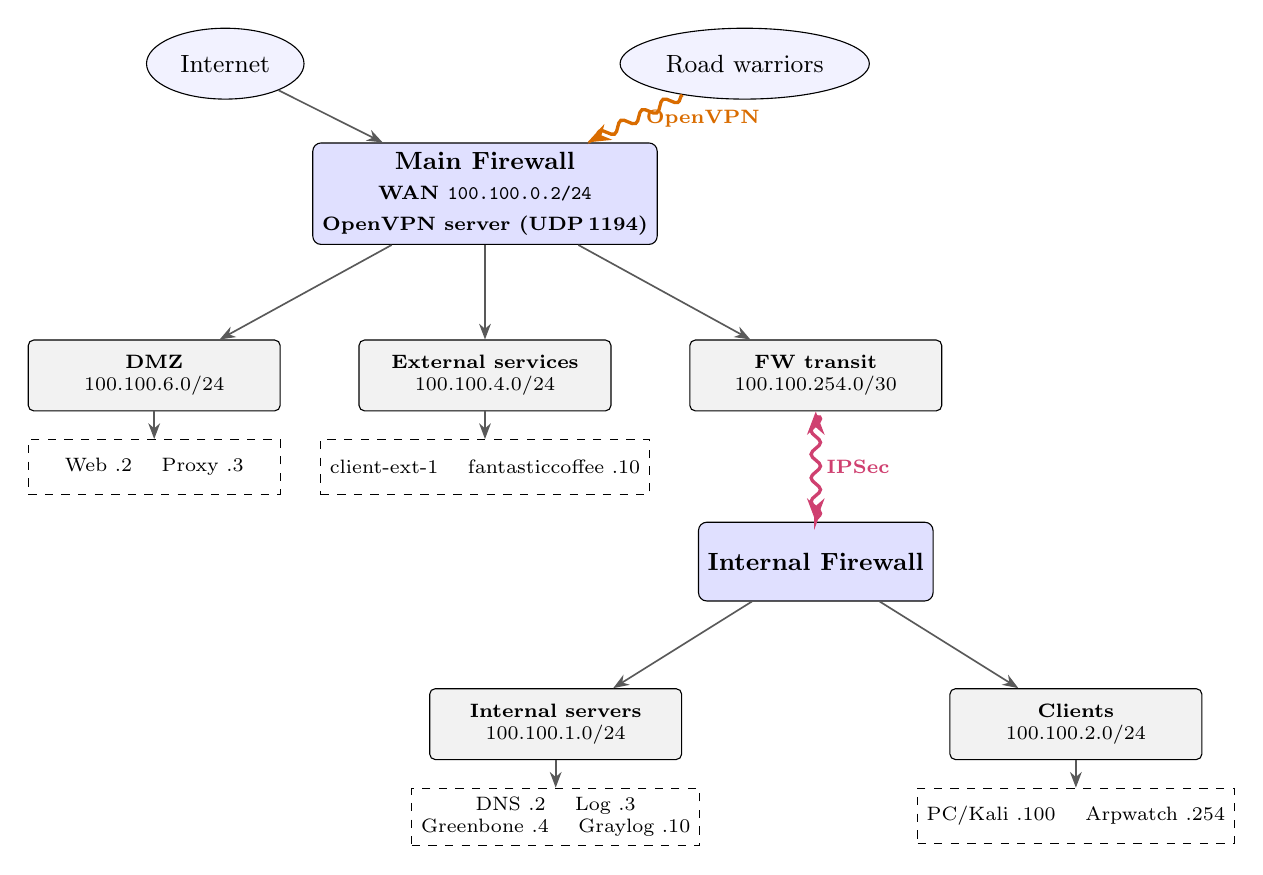
\begin{tikzpicture}[
  font=\sffamily,
  node distance=0.9cm and 1.1cm,
  fw/.style={draw, rounded corners=3pt, fill=blue!12, minimum width=2.8cm,
             minimum height=1cm, align=center, font=\small\bfseries},
  net/.style={draw, fill=gray!10, rounded corners=2pt, minimum width=3.2cm,
              minimum height=0.9cm, align=center, font=\scriptsize},
  host/.style={draw, dashed, fill=white, minimum width=3.2cm,
               minimum height=0.7cm, align=center, font=\scriptsize},
  cloud/.style={draw, ellipse, fill=blue!5, minimum width=2cm,
                minimum height=0.9cm, font=\small},
  link/.style={-Stealth, semithick, draw=black!65},
  vpn/.style={-Stealth, very thick, draw=orange!85!black,
              decoration={snake, amplitude=.6mm, segment length=3mm},
              decorate},
  ipsec/.style={Stealth-Stealth, very thick, draw=purple!75,
                decoration={snake, amplitude=.6mm, segment length=3mm},
                decorate},
]

\node[cloud] (inet) {Internet};
\node[cloud, right=4cm of inet] (rw) {Road warriors};

\node[fw, below=1cm of $(inet)!0.5!(rw)$] (mfw)
    {Main Firewall \\ \scriptsize WAN \texttt{100.100.0.2/24} \\ \scriptsize OpenVPN server (UDP\,1194)};

\node[net, below left=1.2cm and 0.4cm of mfw] (dmz)
    {\textbf{DMZ} \\ 100.100.6.0/24};
\node[net, below=1.2cm of mfw] (ext)
    {\textbf{External services} \\ 100.100.4.0/24};
\node[net, below right=1.2cm and 0.4cm of mfw] (link)
    {\textbf{FW transit} \\ 100.100.254.0/30};

\node[host, below=0.35cm of dmz] (dmzh)
    {Web .2 \quad Proxy .3};
\node[host, below=0.35cm of ext] (exth)
    {client-ext-1 \quad fantasticcoffee .10};

\node[fw, below=1.4cm of link] (ifw) {Internal Firewall};

\node[net, below left=1.1cm and 0.2cm of ifw] (srv)
    {\textbf{Internal servers} \\ 100.100.1.0/24};
\node[net, below right=1.1cm and 0.2cm of ifw] (cli)
    {\textbf{Clients} \\ 100.100.2.0/24};

\node[host, below=0.35cm of srv] (srvh)
    {DNS .2 \quad Log .3 \\ Greenbone .4 \quad Graylog .10};
\node[host, below=0.35cm of cli] (clih)
    {PC/Kali .100 \quad Arpwatch .254};

\draw[link] (inet) -- (mfw);
\draw[vpn] (rw) -- node[midway, right, font=\scriptsize\bfseries, text=orange!85!black] {OpenVPN} (mfw);
\draw[link] (mfw) -- (dmz);
\draw[link] (mfw) -- (ext);
\draw[link] (mfw) -- (link);
\draw[link] (dmz) -- (dmzh);
\draw[link] (ext) -- (exth);
\draw[ipsec] (link) -- node[midway, right, font=\scriptsize\bfseries, text=purple!75] {IPSec} (ifw);
\draw[link] (ifw) -- (srv);
\draw[link] (ifw) -- (cli);
\draw[link] (srv) -- (srvh);
\draw[link] (cli) -- (clih);

\end{tikzpicture}
\caption{ACME-30 topology with the two VPN services introduced in this
assignment: the road-warriors OpenVPN terminates on the WAN interface of
the Main firewall, while the IPSec tunnel protects every packet flowing
on the transit link between the Main and the Internal firewalls.}
\label{fig:topology}
\end{figure*}

\end{document}
